% Drawing 69/01-2 -- folder 69, batch 01, archive page 3 (PDF page 4).
% Transcription: barré avec le Lemme 4 : un triangle de sommets $w$, $u$, $v$, dont les côtés se prolongent en trois demi-droites marquées $\gamma_4$, $\beta_4$, $\alpha_4$
% Kind: struck triangle with extended sides. Method 2 (schematic redraw from the facsimile). Status: partial.
% Notes: Triangle with sides prolonged as half-lines: towards the top left (gamma_4), to the right along the base (beta_4), and down from the lower left vertex (alpha_4, its end outside the label area). Struck by large loops, drawn grey. The vertex letters w, u, v are not legible on the crop and are placed by the transcription.
% Coordinates: 1 unit = 1 mm = 1/100 of the crop width (bbox in page fractions: [0.06, 0.42, 0.5, 0.58]).
% Redrawn by Claude (claude-opus-5-5), issue #73, 2026-11-07; not checked by a human; not compiled (no TeX in the session).
% Rights: reproduces part of the work -- behind RENDER_TRANSCRIPTS, never published by itself.
\documentclass[tikz,border=3pt]{standalone}
\usepackage{amsmath,amssymb}
\usetikzlibrary{patterns,arrows.meta}
\tikzset{pencil/.style={black!45}, struck/.style={black!35}, mark/.style={circle,draw,inner sep=1.3pt}, pt/.style={circle,fill,inner sep=0.9pt}, opt/.style={circle,draw,fill=white,inner sep=1.1pt}}
\begin{document}
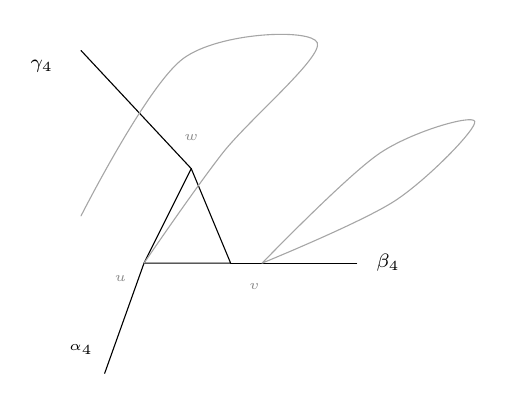
\begin{tikzpicture}[x=1mm,y=1mm,line cap=round,line join=round,font=\scriptsize]
\draw (36,-24) -- (30,-36) -- (41,-36) -- cycle;
\draw (36,-24) -- (22,-9);
\draw (41,-36) -- (57,-36);
\draw (30,-36) -- (25,-50);
\draw[struck] plot[smooth, tension=0.55] coordinates {(22,-30) (35,-10) (52,-8) (40,-22) (30,-36)};
\draw[struck] plot[smooth, tension=0.55] coordinates {(45,-36) (60,-22) (72,-18) (62,-28) (45,-36)};
\node[inner sep=1pt] at (17,-11) {\scriptsize $\gamma_4$};
\node[inner sep=1pt] at (61,-36) {\scriptsize $\beta_4$};
\node[inner sep=1pt] at (22,-47) {\tiny $\alpha_4$};
\node[inner sep=1pt,pencil] at (36,-20) {\tiny $w$};
\node[inner sep=1pt,pencil] at (27,-38) {\tiny $u$};
\node[inner sep=1pt,pencil] at (44,-39) {\tiny $v$};
\end{tikzpicture}
\end{document}
